\documentclass[12pt,a4paper,titlepage,headinclude,bibtotoc]{scrartcl}

%---- Allgemeine Layout Einstellungen ------------------------------------------

% Für Kopf und Fußzeilen, siehe auch KOMA-Skript Doku
\usepackage[komastyle]{scrpage2}
\pagestyle{plain}
\setheadsepline{0.5pt}[\color{black}]
\automark[section]{chapter}


%Einstellungen für Figuren- und Tabellenbeschriftungen
\setkomafont{captionlabel}{\sffamily\bfseries}
\setcapindent{0em}


%---- Weitere Pakete -----------------------------------------------------------
% Die Pakete sind alle in der TeX Live Distribution enthalten. Wichtige Adressen
% www.ctan.org, www.dante.de

% Sprachunterstützung
\usepackage[ngerman]{babel}
\usepackage{caption}
% Benutzung von Umlauten direkt im Text
% entweder "latin1" oder "utf8"
\usepackage[utf8]{inputenc}

% Pakete mit Mathesymbolen und zur Beseitigung von Schwächen der Mathe-Umgebung
\usepackage{latexsym,exscale,stmaryrd,amssymb,amsmath}


\usepackage[nointegrals]{wasysym}
\usepackage{eurosym}

% Anderes Literaturverzeichnisformat
%\usepackage[square,sort&compress]{natbib}
\usepackage{hyperref}
% Für Farbe
\usepackage{color}
\usepackage{graphicx}
\usepackage{wrapfig}
\usepackage{subfigure}

% Caption neben Abbildung
\usepackage{sidecap}


% Befehl für "Entspricht"-Zeichen
\newcommand{\corresponds}{\ensuremath{\mathrel{\widehat{=}}}}
% Befehl für Errorfunction
\newcommand{\erf}[1]{\text{ erf}\ensuremath{\left( #1 \right)}}


%Fußnoten zwingend auf diese Seite setzen
\interfootnotelinepenalty=1000

%Für chemische Formeln (von www.dante.de)
%% Anpassung an LaTeX(2e) von Bernd Raichle
\makeatletter
\DeclareRobustCommand{\chemical}[1]{%
  {\(\m@th
   \edef\resetfontdimens{\noexpand\)%
       \fontdimen16\textfont2=\the\fontdimen16\textfont2
       \fontdimen17\textfont2=\the\fontdimen17\textfont2\relax}%
   \fontdimen16\textfont2=2.7pt \fontdimen17\textfont2=2.7pt
   \mathrm{#1}%
   \resetfontdimens}}
\makeatother
\usepackage{textcomp}
\usepackage{upgreek}
%\begin{document}
%$\upmu$
%\end{document}
%Honecker-Kasten mit $$\shadowbox{$xxxx$}$$
\usepackage{fancybox}

%SI-Package
\usepackage{siunitx}

%keine Einrückung, wenn Latex doppelte Leerzeile
\parindent0pt

%Bibliography \bibliography{literatur} und \cite{gerthsen}
%\usepackage{cite}
\usepackage{babelbib}
\selectbiblanguage{ngerman}

\usepackage{siunitx}
%\begin{document}
 % \SI{1.55}{\micro\metre}
\sisetup{math-micro=\text{µ},text-micro=µ}
\usepackage{amsmath}

\usepackage[verbose]{placeins}
%für \FloatBarrier

\begin{document}

\begin{titlepage}
\centering
\textsc{\Large Physikalisch- Chemisches Grundpraktikum\\[1.5ex] Universität Göttingen}

\vspace*{0.5cm}

\rule{\textwidth}{1pt}\\[0.5cm]
{\huge \bfseries
  Ersatzversuch: \\[1.5ex]
Neutralisationsenthalpie }\\[0.5cm]
\rule{\textwidth}{1pt}

\vspace*{0.5cm}


\begin{Large}
\begin{tabular}{ll}
Durchführende: &  Isaac Maksso, Julia Stachowiak\\
Assistent: & Marvin \\
 Versuchsdatum: & 24.11.2016\\
 Datum der ersten Abgabe: & 1.12.2016\\
\end{tabular}
\end{Large}

\vspace*{0.5cm}

\end{titlepage}


\tableofcontents

\section{Experimentelles}
\subsection{Versuchsaufbau}


\begin{figure}[h]
\centering
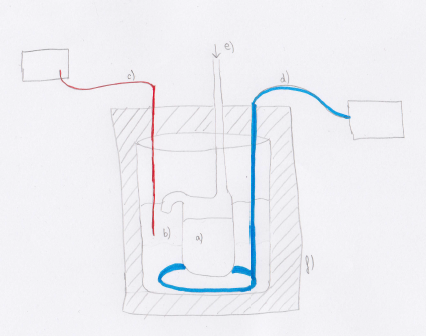
\includegraphics[scale=1]{Versuchsbau.png}
\caption{Der Versuchsaufbau (ohne die Kalibrierungsmessung für das Thermoelement).}
\end{figure} 
\FloatBarrier

a) Gefäß mit $HCl$ bzw. $HAc$\\
b) Becherglas mit $NaOH$ bzw. $H_2O$\\
c) Thermoelement\\
d) Tauchsieder\\
e) Pumpe \\
f) näherungsweise adiabatischer Mantel (Styropor und doppelwandiges Glasgefäß)\\


\subsection{Durchführung}
Die Neutralisationsenthalpie von $HCl$ und $HAc$ sollten mittels der Verdünnungsenthalpie von $HCl$ bestimmt werden. Der Versuch bestand aus 3 Durchläufen. In den ersten beiden Durchläufen wurden $HCl$ und $HAc$ mit $NaOH$ neutralisiert, im 3. Durchlauf $HCl$ mit Wasser verdünnt.\\
Zuerst wurde ein Überschuss (grob $2g$) $NaOH$ in ein Becherglas abgewogen, in dem. Wasser gelöst und in das Isolationsgefäß gestellt. Außerdem wurden jeweils ca. 20 ml Säure in ein Glasgefäß gefüllt und dieses in die Lauge gestellt.
Während der 5-minütigen Vorlaufphase sollten beide Gefäße die gleiche Temperatur erreichen. Anschließend wurde mittels Pumpe die innere Flüssigkeit zu der äußeren befördert; die Nachphase verlief analog zur Vorphase. Während der ganzen Zeit wurde die Temperaturdifferenz mittels Theroelement aufgezeichnet. \\
Da die Wärmekapazität temperatur- und stoffabhängig ist, wurde diese jeweils im Anschluss bestimmt. Dies geschah über die Zufuhr einer definierten Wärmemenge mittels Tauchsieder über $t=100$ s bei $U= 12-13$ V und $I=14-15$ mA über $\Delta T=100$ s. Analog zum 1. Teil wurde die Temperaturdifferenz über die Zeit für Vorlauf- Haupt- und Endphase bestimmt. \\
Um die Messergebnisse des Thermoelements zu korrigieren, wurden beim ersten Versuch Temperatur und Spannung manuell per Beckmannthermometer bzw. Voltmeter alle 30 s abgelesen. Mit der daraus bestimmten Kalibriergerade konnte für die nächsten Durchgänge mit Werten der Genauigkeit des Beckmannthermometers und Voltmeters gerechnet werden, ohne dass diese manuell abgelesen werden mussten.  Ebenfalls wurden Spannung und Stromstärke alle 30 s notiert, um sicherzustellen, dass keine Schwankungen das Ergebnis verfälschen.\\
Das Glasgefäß mit der Säure wurde vor und nach dem Versuch genau gewogen um die genaue Masse an Säure zu ermitteln, die involviert war.\\

\newpage
\section{Auswertung}
Die Temperatur-Zeit-Diagramme sind im Anhang zu finden. Besonders während der Vor- und Nachphase ist zu sehen, dass der Vorgang nicht ideal-adiabatisch verlief, da Wärme entweichen konnte und die Linien nicht gerade verlaufen. Bei Abbildung (\ref{HClundNaOH}) ist kurz vor Zusammenführung beider Flüssigkeiten ein Temperaturabfall zu sehen. Dies kann von einer ungleichmäßigen Wärmeverteilung durch den Rührfisch am Thermoelement kommen, besonders weil dieser Sprung nicht bei der Aufzeichung der Temperaturen mittels Beckmannthermometer zu sehen ist. Der kurze $"$Peak$"$ bei Abbildung (\ref{HClundNaOH}) und (\ref{HAcundNaOH}) kommt ebenfalls wahrscheinlich von einer kurzen unregelmäßigen Wärmeverteilung am Thermoelement.\\

\subsection{Bestimmung der Wärmekapazität}

Bei konstantem Druck fällt der letze Term von $dH$ weg und aus dem ersten Hauptsatz der Thermodynamik ergibt sich die in Gleichung (\ref{1.HS}) und (\ref{C_p}) gezeigte Beziehung.

\begin{equation} \label{1.HS}
dU= \delta Q+ \delta W= dH- pdV
\end{equation}

\begin{equation}\label{C_p}
C_{\mathit{m},p}= \left(\frac{\delta Q}{\partial T}\right)_p =\left(\frac{\partial H}{\partial T}\right)_p
\end{equation}

Der erste Hauptsatz der Thermodynamik ($dU= \delta Q \cdot \delta W$) gilt für geschlossene Systeme, d.h. für Systeme mit Energie- aber ohne Stoffaustausch mit der Umgebung. Das Gefäß mit $HCl$ sowei das Gefäß mit $NaOH$ sind jeweils (annähernd) adiabatische Gefäße, die zusammen ein abgeschlossenes System bilden. Daher kann der 1. Hauptsatz hier für die Berechnung verwendet werden. Die Änderung der inneren Energie bzw. Enthalpie bezieht sich auf die Gesamtheit beider Flüssigkeiten, die miteinander in Kontakt gebracht werden, d.h. ein abgeschlossenes System bilden. Der Lufteinstrom durch die Pumpe ist an dieser Stelle zu vernachlässigen.\\

Die Berechnung von $C_p$ erfolgte jeweils über die 2. Versuchsphase nach Gleichung (\ref{C_pFormel}). Hier wurde $\Delta Q_{\mathrm{el}}= U\cdot I \cdot \Delta t$ in Gleichung (\ref{C_p}) eingesetzt. Die Temperaturdifferenzen wurden aus den Graphen durch lineare Extrapolation ermittelt. Die Ergebnisse sind in Tabelle (\ref{C_pTabelle}) dargestellt.\\

\begin{equation} \label{C_pFormel}
C_p=\frac{U\cdot I\cdot \Delta t}{\Delta T}
\end{equation}

\FloatBarrier
\begin{table} \caption{Berechnete Werte für $C_p$}
\label{C_pTabelle} 
\begin{tabular}{c|c|c} 
&$\Delta T$ [K] &$C_p$ [J/K]\\
\hline
$HCl/NaOH$&2,286&794,7\\
\hline	
$HAc/HaOH$&2,087&871,6\\
\hline
$HCl$ Verdünnung&1,94&937\\
\end{tabular} 
\end{table}

 
Um die molare Wärmekapazität zu ermitteln, muss die Stoffmenge der Flüssigkeiten errechnet werden. Diese setzt sich zusammen aus der Stoffmenge der gelösten Ionen und des Wassers. Erstere berechnet sich nach Gleichung (\ref{n}). Die sich daraus ergebende Masse von der Gesamtmasse subtrahiert ergibt die reine Masse(bzw. umgerechnet Stoffmenge) des Wassers. Die Ergebnisse sind in Tabelle (\ref{StoffmengenTabelle}) dargestellt.
 
\begin{equation}\label{n}
n=\frac{c \cdot m}{\rho}
\end{equation}

\begin{table} \caption{Stoffmengen und die molare Wärmakapazität $C_{\mathrm{m},p}$}
\label{StoffmengenTabelle} 
\begin{tabular}{c|c|c|c|c}
&$n_\mathrm{Ionen}$& $n_{H_2O}$&$n_\mathrm{ges}$&$C_{\mathrm{m},p}$[J$\cdot \mathrm{mol}^{-1}\cdot \mathrm{K}^{-1}$]\\
\hline
$HCl/NaOH$&0,03958019&1,051390&1,090970&728,3926\\
\hline	
$HAc/HaOH$&0,03933589&0,9772290&1,016565&857,3930\\
\hline
$HCl$ Verdünnung&0,03912718&1,039356&1,078483&868,3672\\
\end{tabular} 
\end{table}
\FloatBarrier

Zur Bestimmung der Verdünnungsenthalpie $\Delta_\mathrm{verd}$ von $HCl$ wurde die Temperaturdifferenz mittels linearer Extrapolation aus Abbildung (\ref{Verduennung}) bestimmt. Mittels der Wärmekapazität konnte die molare Neutralisationsenthalpie nach Gleichung (\ref{C_p}) bestimmt werden. Da bei der Neutralisation ebenfalls auch eine Verdünnung stattfindet, muss diese pro mol von der gemessenen Reaktionsenthalpie abgezogen werden (Gleichung \ref{Neutralisationsenthalpie}). Die Ergebnisse beider Rechnungen sind in Tabelle (\ref{TabelleVerdNeutr}) dargestellt.\\
Die Verdünnungsenthalpie von $HAc$ ist nicht bekannt. Da die Verdünnungsenthalpien für verschiedene Säuren ungefähr gleich sind, wurde zur Berechnung die $\Delta H_\mathrm{verd}(HCl)$ verwendet.\\

\begin{equation}\label{Neutralisationsenthalpie}
\Delta H_\mathrm{m, N}= \frac{\Delta H_\mathrm{R}}{n_{HCl \mathrm{V1}}}- \frac{\Delta H_\mathrm{verd}}{n_{HCl \mathrm{V3}}} 
\end{equation}

\begin{equation}\label{n}
n=\frac{c \cdot m}{\rho}
\end{equation}

\begin{table} \caption{Verdünnungs- und Neutralisationsenthalpie}
\label{TabelleVerdNeutr} 
\begin{tabular}{c|c|c|c|c}
& $\Delta H_\mathrm{R}$ &  $\Delta H_\mathrm{R}$  & $\Delta H_\mathrm{m, verd}$  &$\Delta H_\mathrm{m, N}$ \\
&[$\mathrm{J}\cdot \mathrm{K}^{-1}$]&[$\mathrm{J}\cdot \mathrm{K}^{-1} \cdot \mathrm{mol}^{-1}$]&[$\mathrm{J}\cdot \mathrm{K}^{-1} \cdot \mathrm{mol}^{-1}$]&[$\mathrm{J}\cdot \mathrm{K}^{-1} \cdot \mathrm{mol}^{-1}$]\\
\hline
$HCl/NaOH$&-1973&-4985$\cdot 10^1$&&-4701$\cdot 10^1$\\
$HAc/NaOH$&-1932&-4912$\cdot 10^1$&& -4629$\cdot 10^1$\\
$HCl$ Verdünnung&-111&-284$\cdot 10^1$&-284$\cdot 10^1$&\\
\end{tabular} 
\end{table}



\subsection{Fehlerrechnung}

\subsection{Bestimmung von $\Delta H_\mathrm{N}$ nach Hess und Vergleich mit Messwerten}

Die Enthalpie einer Reaktion ergibt sich aus der Differenz der Standardbildungsenthalpien $H_f$ der Produkte und Edukte.

\begin{equation}
\Delta H_\mathrm{R}= \sum_i \nu_i H_\mathrm{Produkte}- \sum_i \nu_i H_\mathrm{Edukte}
\end{equation}

\begin{equation}
H^+_{(aq)} + OH^-_{(aq)} \rightleftharpoons H_2O_{(l)}
\end{equation}

\begin{equation}
\Delta H_\mathrm{N}= H_\mathrm{f}(H_2O_{(l)}) -H_\mathrm{f}(H^+_{(aq)}) -H_\mathrm{f}(OH^-_{(aq)}) = -55,815\, \mathrm{kJ}\cdot \mathrm{mol}^{-1}
\end{equation}

Mit $H_\mathrm{f}(H_2O_{(l)})$ = -285,830 kJ $\cdot \mathrm{mol}^{-1}$\footnote{Haynes, W.M.: \emph{Handbook of Chemistry and Physics}, CRC Press, Boca Raton, London, New Yorck, \textbf{2014}.}\\
$H_\mathrm{f}(H^+_{(aq)})$= 0 kJ $\cdot {\mathrm{mol}^{-1}}^1$\\
$H_\mathrm{f}(OH^-_{(aq)})$ = -230,015 kJ $\cdot {\mathrm{mol}^{-1}}^1$\\

Die Neutralisationsenthalpie weicht für $HCl$ und $HAc$ um ca. $-20\%$ vom Literaturwert ab. 
\textbf{Fehlergrenzen}
Die systematischen Fehler werden ausführlich in der Diskussion diskutiert.\\

Da die Wärmekapazitäten stark konzentrations- und temperaturabhängig sind, können hier keine vergleichbaren Literaturwerte gefunden werden.\\

\section{Diskussion systematischer Fehler}
Eine erste Messungenauigkeit ist die Kalibrierung des Thermoelements. Spannung und Temperatur wurden über den ersten Versuch hinweg notiert, und die Werte für Vor- und Nachphasen aufgetragen. Die sich ergebene Geradengleichung gibt für jede gemessene Spannung die Temperatur an, die das Beckmannthermometer nach dieser Messung anzeigen würde. Die Bestimmung der Kalibrierkurve hat einen besonderen Anspruch an Genauigkeit, da damit die Temperaturwerte des Themoelements für die anderen Messungen umgerechnet wurden. Jedoch ist diese Messung sehr fehlerbelastet: Das Ablesen von Spannung und Temperatur geschah nicht genau gleichzeitig und nicht genau alle 30\,s und das Beckmannthermometer braucht jeweils kurz Zeit um sich einzustellen. Wie in der Auftragung zu sehen ist, liegen auch die Werte leicht gestreut. Die sich ergebenen Fehler der Kalibrierkurve wurden in der Fehlerrechnung \textbf{berücksichtigt} oder \textbf{nicht berücksichtigt}.\\

Ebenfalls fehlerbehaftet sind die Ermittlungen der Wärmekapazitäten. Spannung und Stromstärke schwankten während der Heizphase zum Glück kaum. Allerdings betrug $\Delta t$ nicht immer genau 100 s, da das Gerät manuell aus- und eingeschaltet wurde. Eine längere Heizrate führt zu größerer Temperaturdifferenz und damit zu einer geringeren Wärmekapazität. Eine zu geringe Wärmekapazität führt wiederum zu einer ebenfalls zu kleinen Enthalpie, wie auch bei dem Versuch gemessen.\\

Eine gleichmäßige Temperaturverteilung (für die ein Rührfisch sorgen sollte) ist zur Ermittlung der richtigen Temperaturerhöhung sehr wichtig. Jedoch ist an den Graphen zu sehen, dass kurzfristig sehr hohe Temperaturen am Thermoelement entstanden und sich später erst wieder verteilten. So kann es auch sein, dass sich die Elektrode des Thermoelemts zu nah am Tauchsieder befand und das umliegende Wasser schneller erwärmt wurde als andere Teile. Dies würde ebenfalls zu einem zu großen $\Delta T$ und damit zu einer zu geringen Wärmekpazität und auch Enthalpie führen. Sollte dies eine signifikante Fehlerquelle darstellen, so müsste die Gerade der Nachphase der Messung stärker abfallen als in der Vorphase. Dieser Effekt ist im Graphen nur leicht zu sehen.\\

Ein großer systematischer Fehler ist der nicht ideal adiabatische Mantel, was auch an den abfallenden Geraden in Anfangs- und Endphase der Auftragungen zu sehen ist. Dies betrifft besonders die Bestimmungen der Wärmekapazität, da hier während der Wärmezufuhr schon wieder Wärme entweichen konnte. Dieser Fehler wird durch die graphische Extrapolation ausgeglichen, da die ermittelte Temperaturdifferenz größer ist als die Temperaturdifferenz, die sich nur aus Betrachtung von Anfangs- und Endpunkt ergäbe. 
Da sich im Vergleich zu den Literaturwerten eine geringere Enthalpie aus den Messwerten ergeben hat, war die Wärmekapazität ebenfalls zu gering und die gemessene Temperaturdifferenz zu groß. Die starke Abweichung kann denmach insbesonders durch diesen systematischen Fehler erklärt werden.\\

%Die Verdünnungsenthalpie von $HAc$ wurde nicht ermittelt, stattdessen wurde mit der Verdünnungsenthalpie von $HCl$ gerechnet. Da $HAc$ im Vergleich jedoch eine schwache Säure ist, muss auch die Verdünnungsen

\newpage
\section{Anhang}

\begin{figure}[h] \label{Kalibrierkurve Thermoelement}
\centering
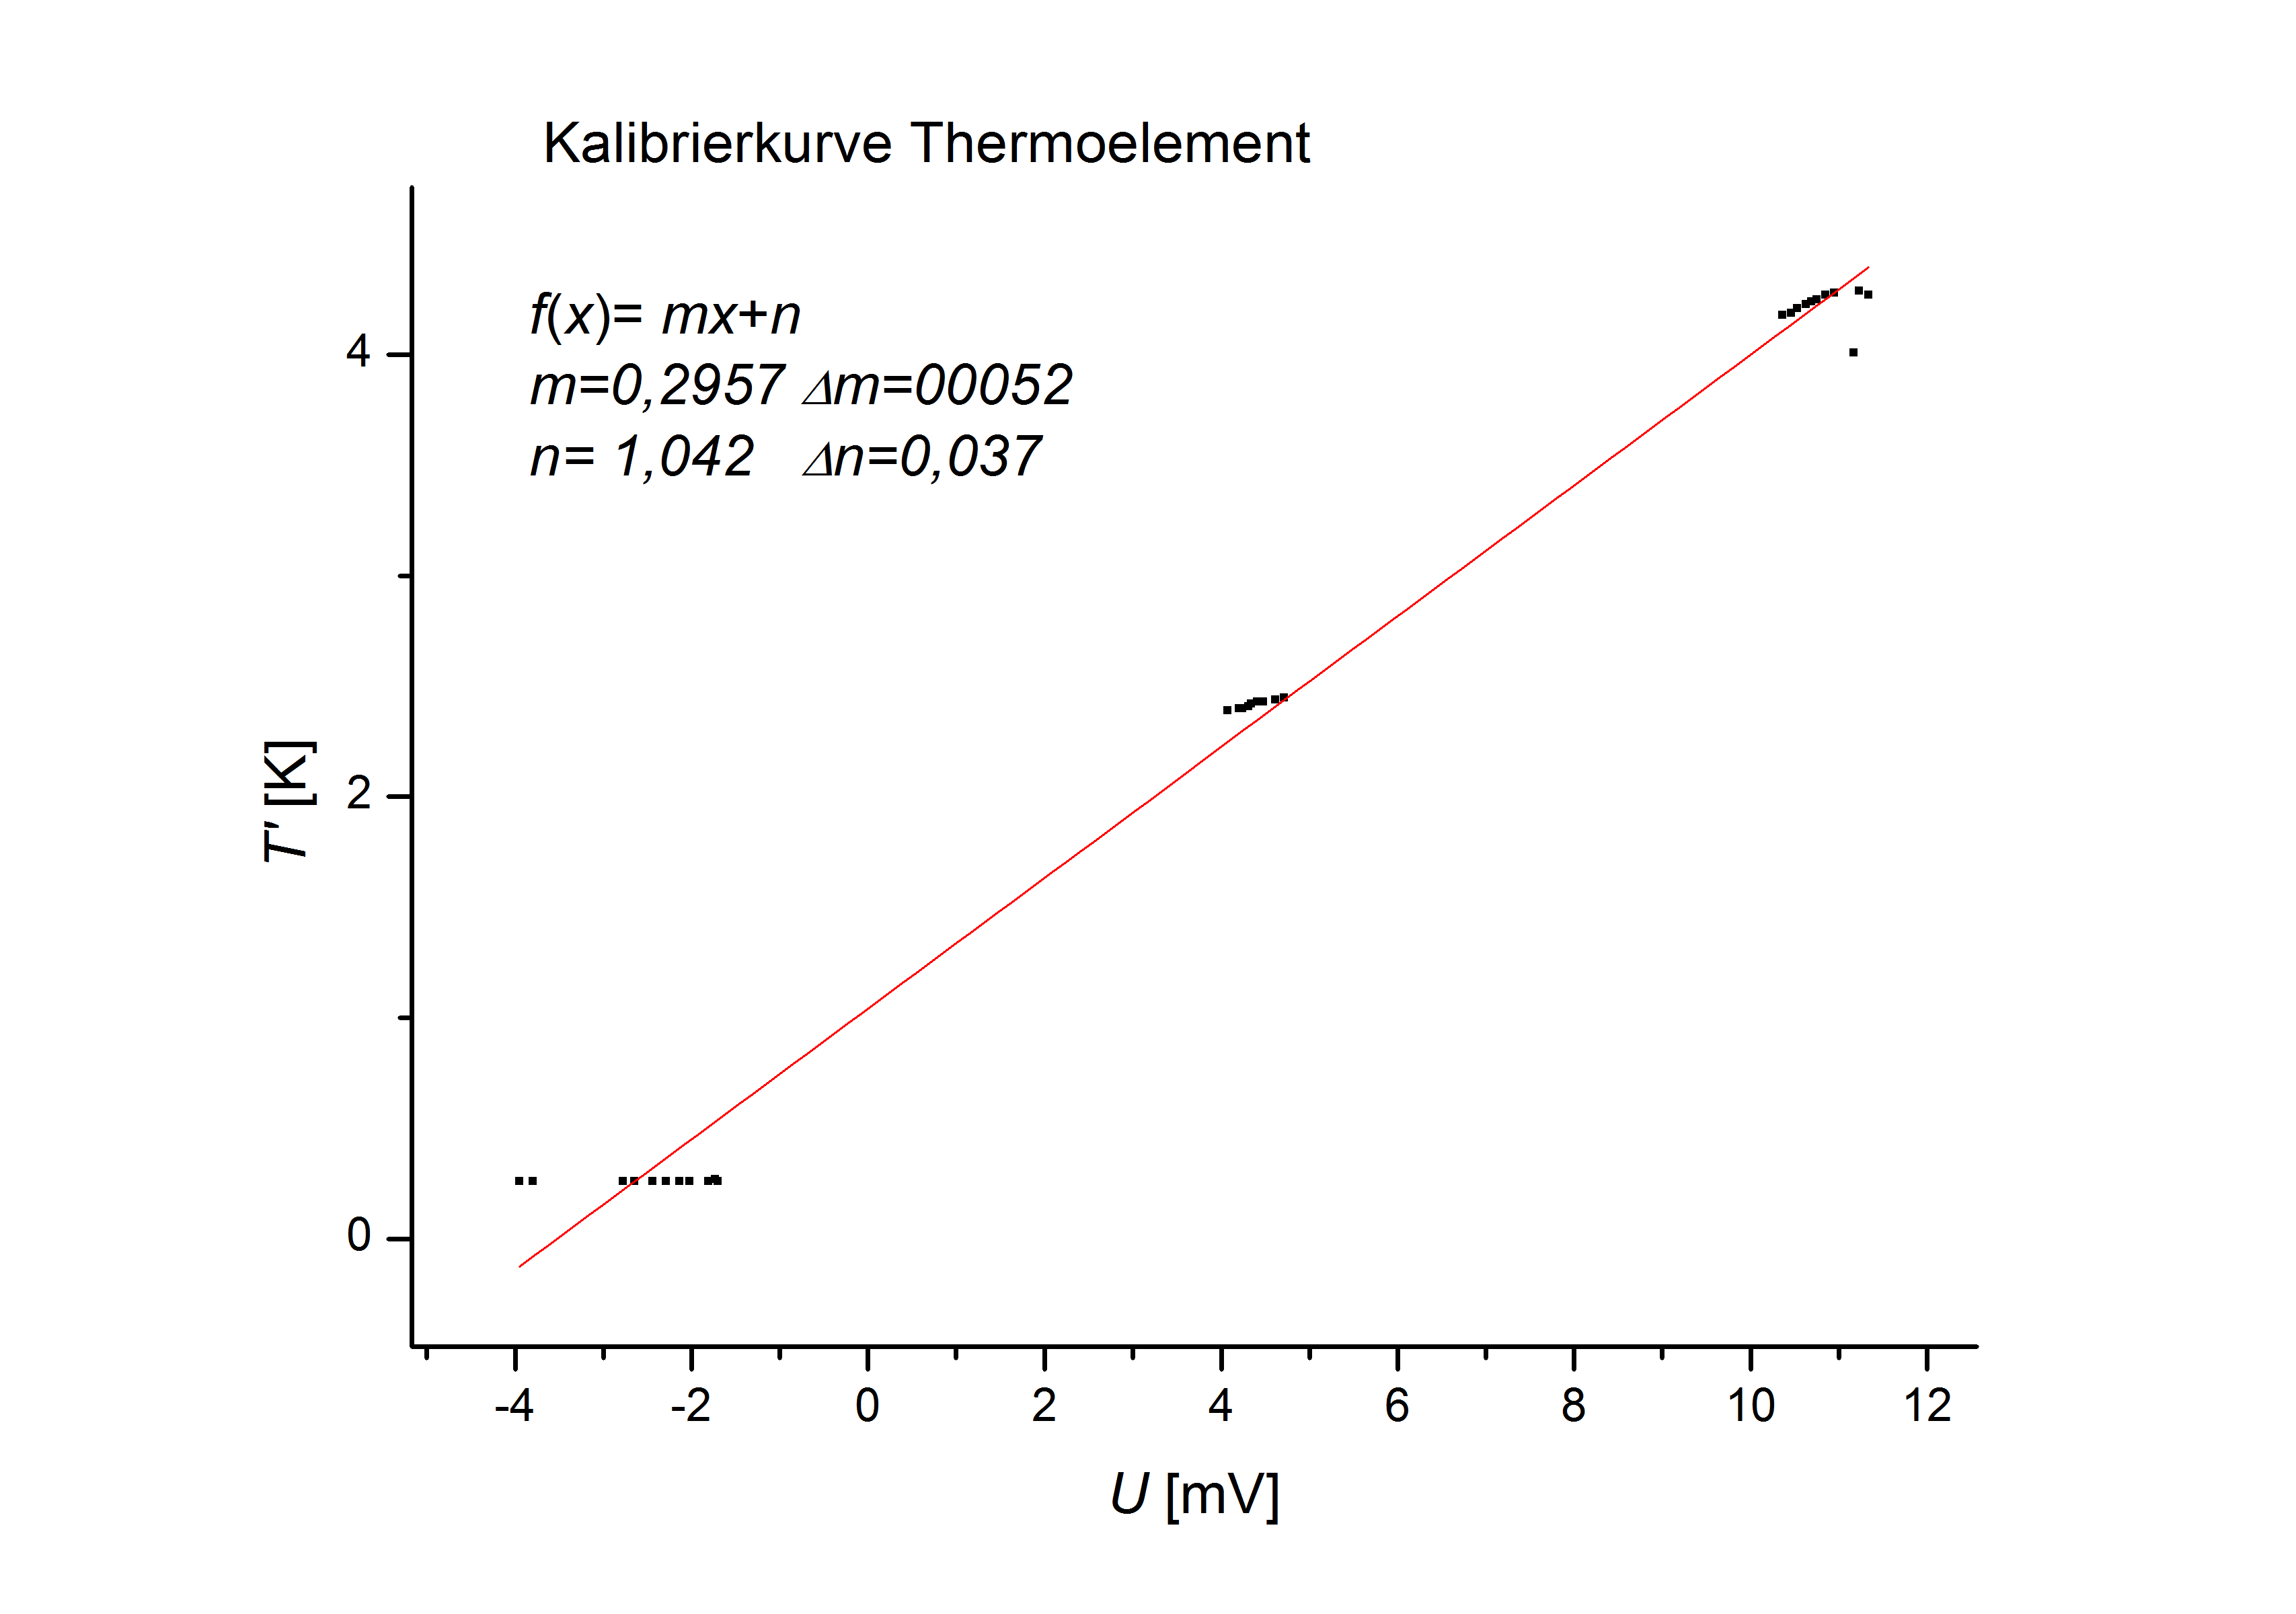
\includegraphics[width=13.5cm]{KalibrierkurveThermoelementOrigin.png}
\caption{Kalibrierkurve des Thermoelements.}
\end{figure} 
\FloatBarrier



\begin{figure}[h] \label{HClundNaOH}
\centering
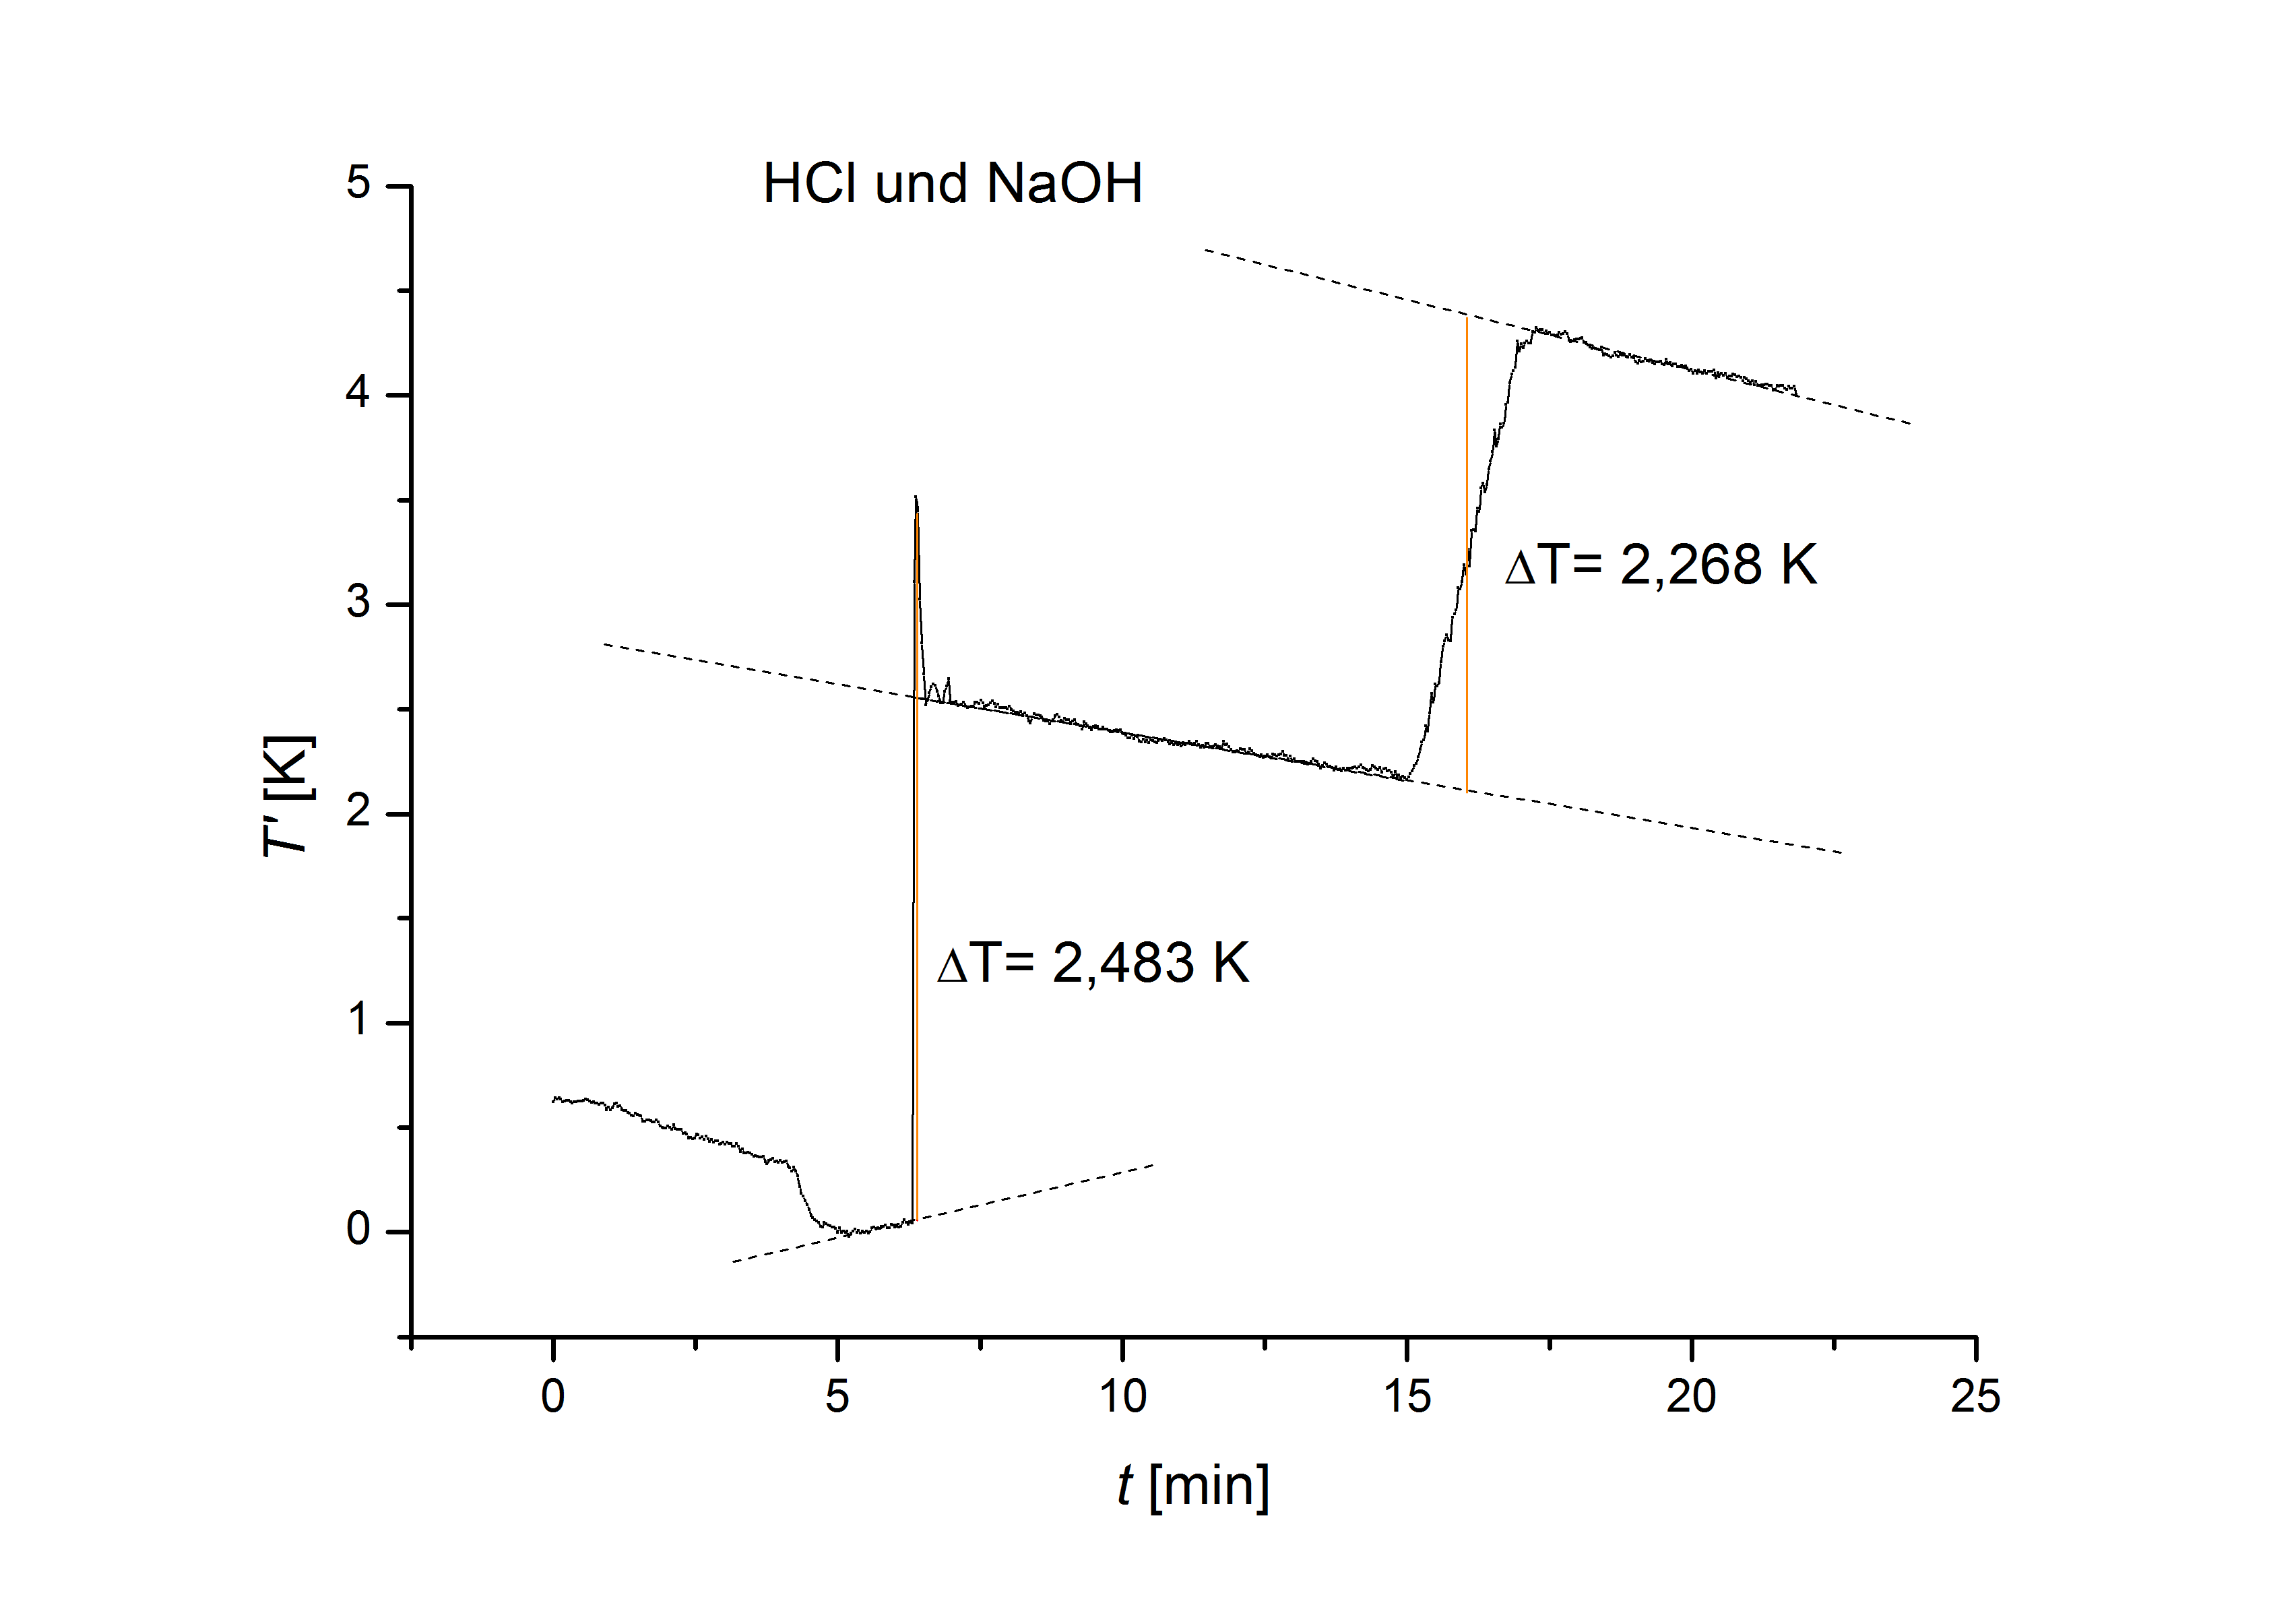
\includegraphics[width=13.5cm]{HClundNaOH.png}
\caption{Temperatur-Zeit Diagramm $HCl$ und $NaOH$.}
\end{figure} 
\FloatBarrier


\begin{figure}[h] \label{HAcundNaOH}
\centering
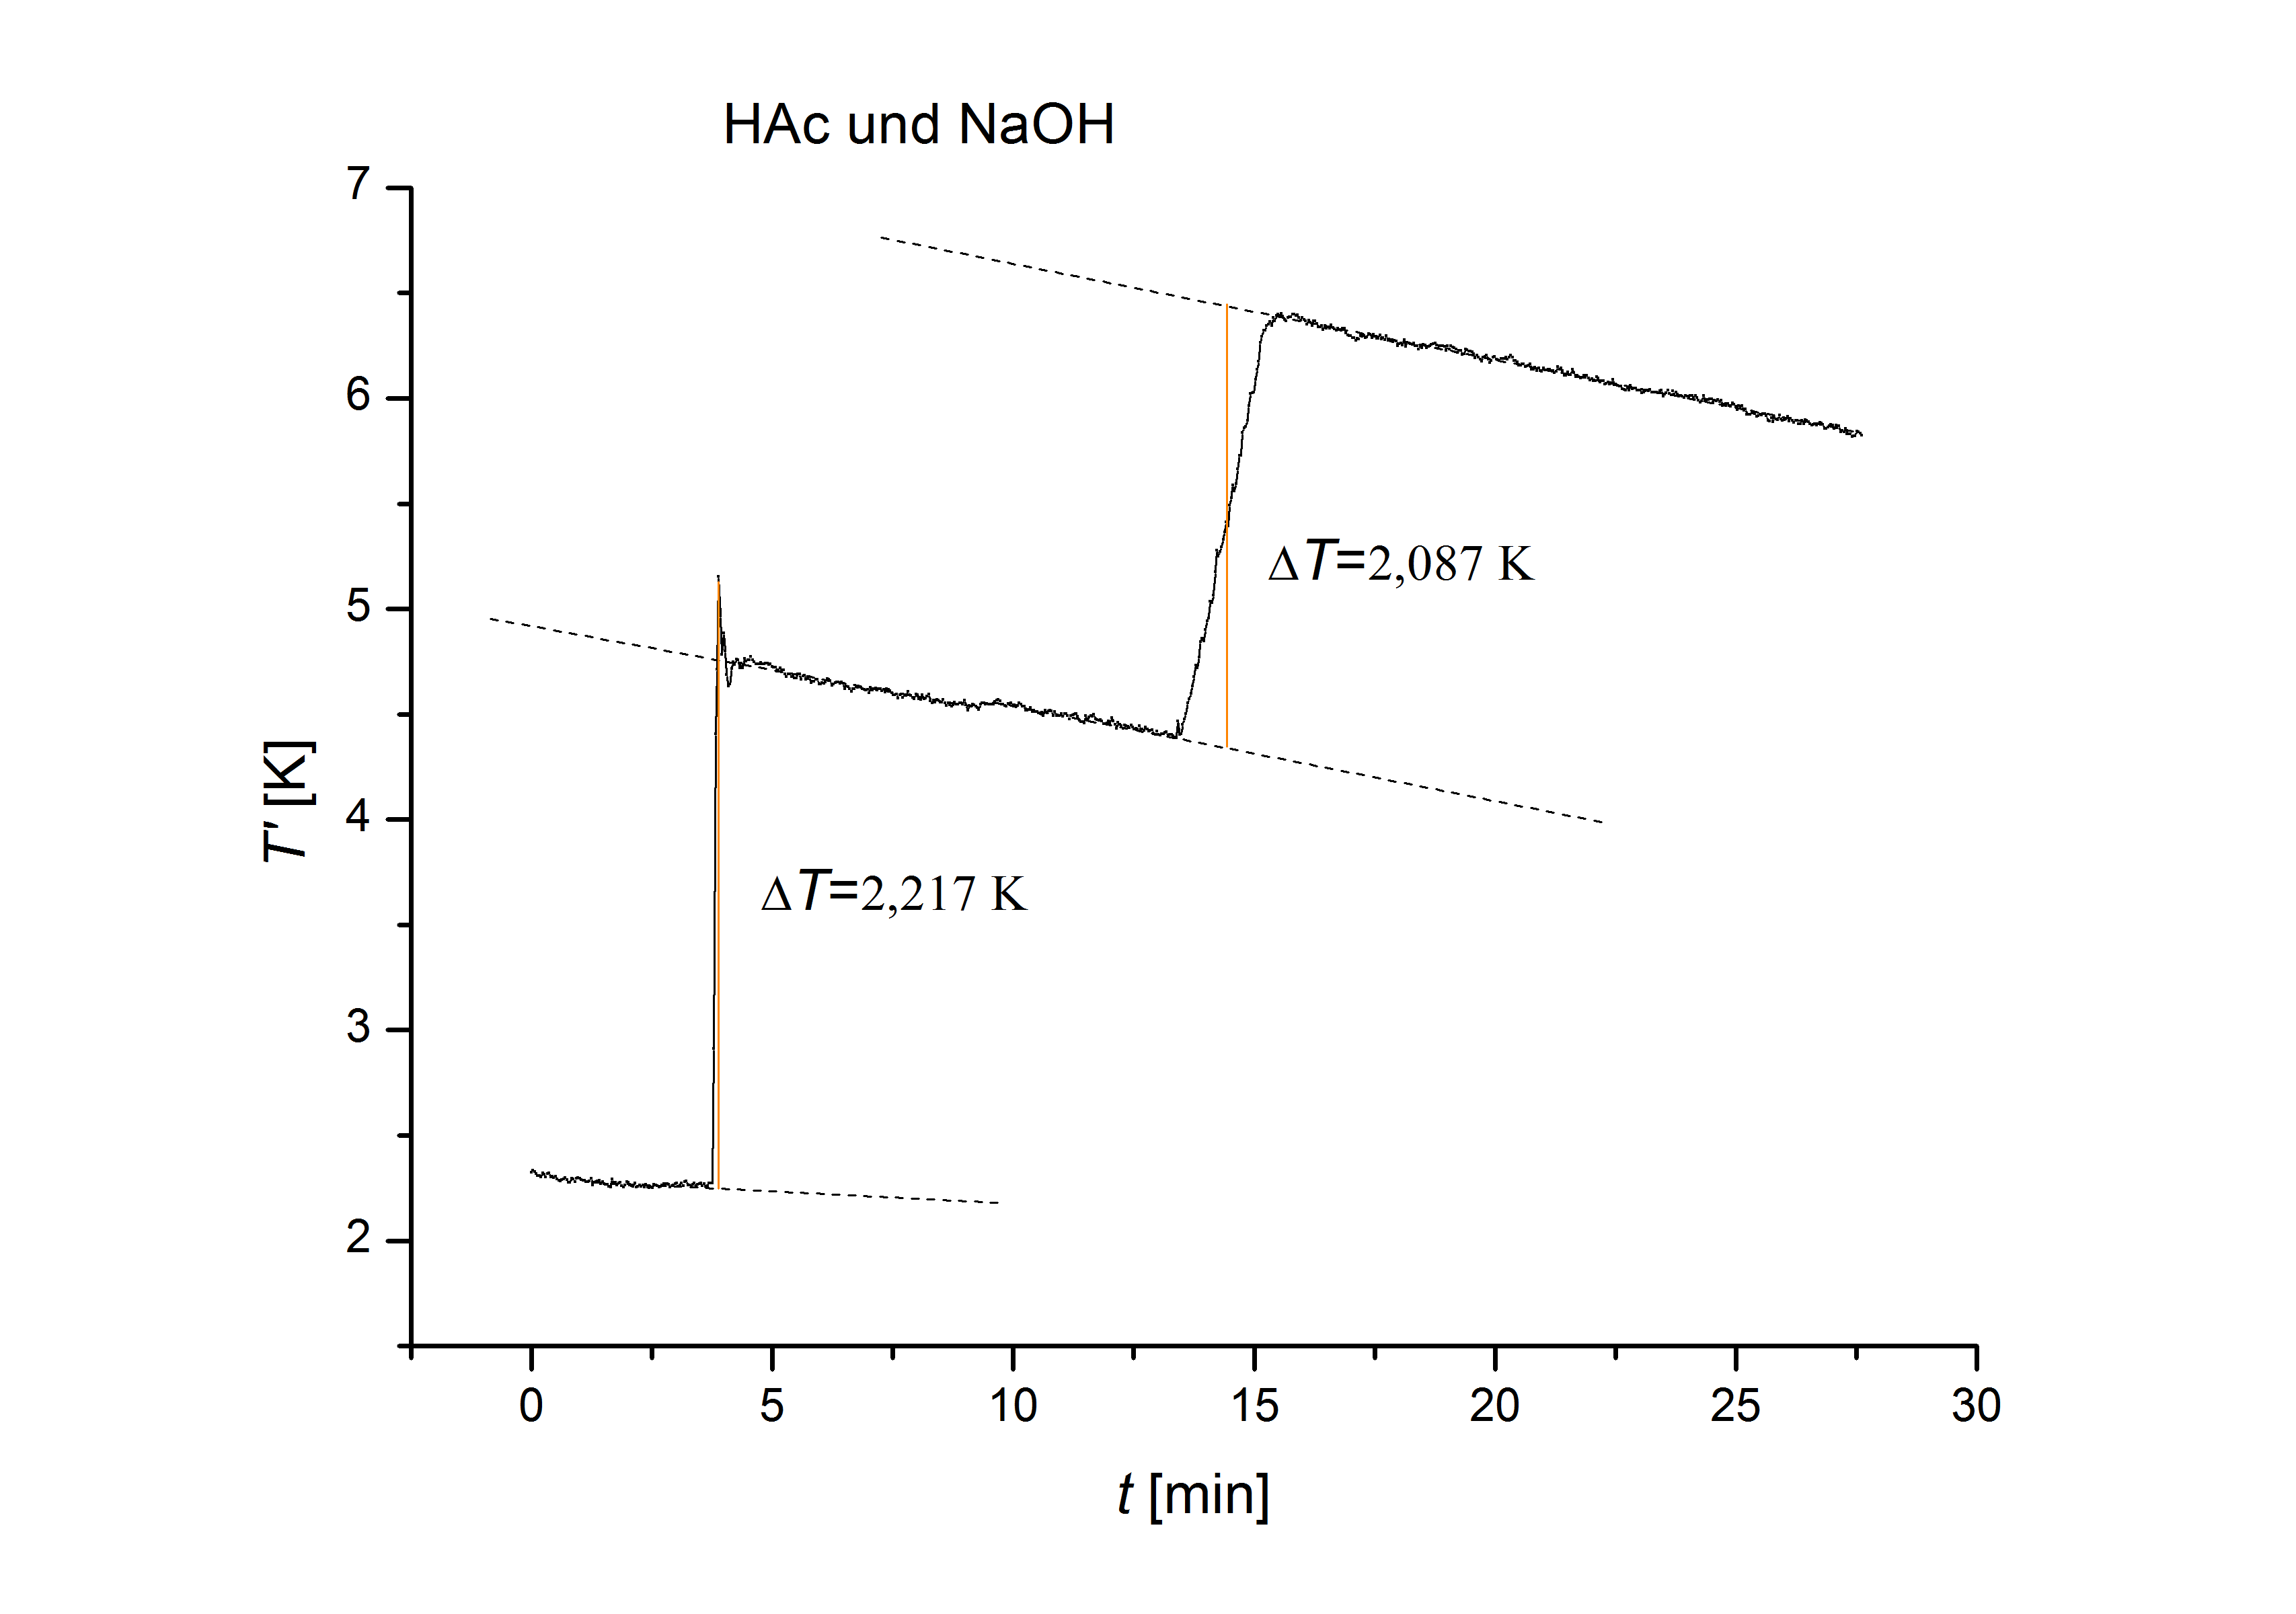
\includegraphics[width=13.5cm]{HAcundNaOH.png}
\caption{Temperatur-Zeit Diagramm $HAc$ und $NaOH$.}
\end{figure} 
\FloatBarrier

\begin{figure}[h]\label{Verduennung}
\centering
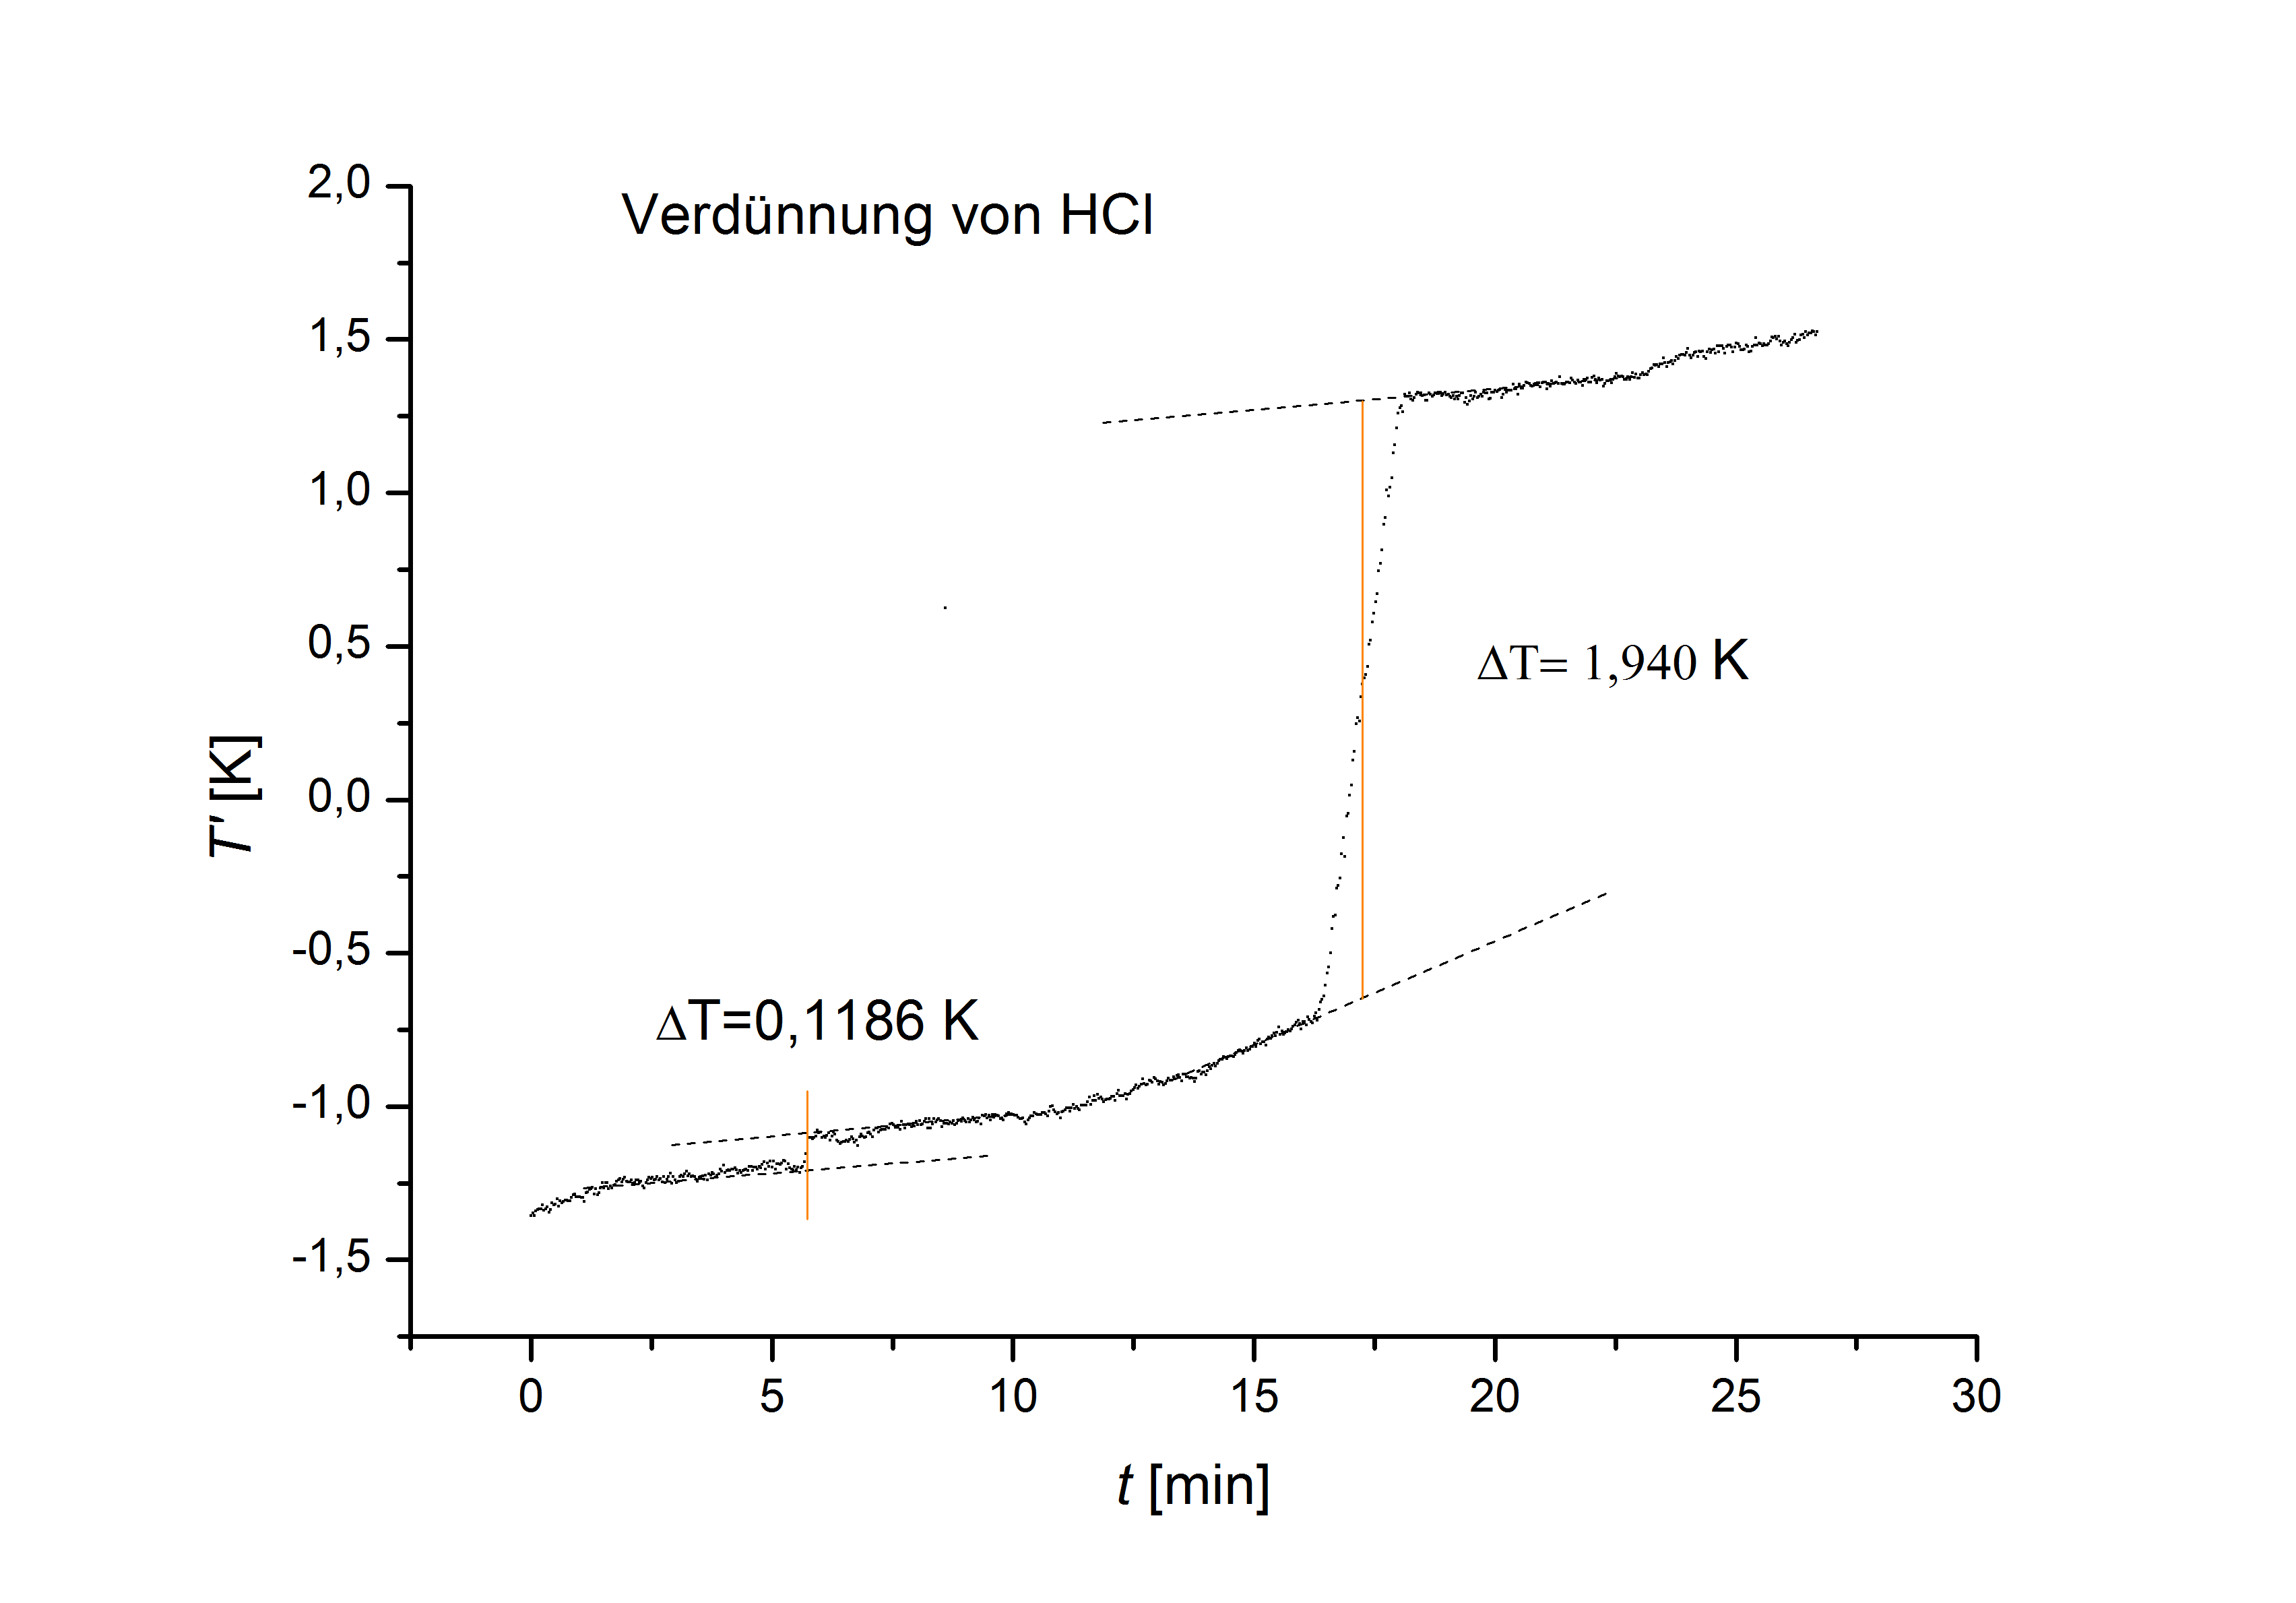
\includegraphics[width=13.5cm]{Verduennungsenthalpie.png}
\caption{Verdünnung von $HCl$.}
\end{figure} 
\FloatBarrier




\section{Literaturverzeichnis}
1\quad Eckhold, Götz: \emph{Praktikum I zur Physikalischen Chemie}, Institut für Physikalische Chemie, Uni Göttingen, \textbf{2014}.
\vspace{0,5 cm}

2 \quad Eckhold, Götz: \emph{Statistische Thermodynamik}, Institut für Physikalische Chemie, Uni Göttingen, \textbf{2012}.

\vspace{0,5cm}

3 \quad Eckhold, Götz: \emph{Chemisches Gleichgewicht}, Institut für Physikalische Chemie, Uni Göttingen, \textbf{2015}.\\

\end{document}


